\documentclass{llncs}

\usepackage{graphicx}
\usepackage{float}
\usepackage{verbatim}
\usepackage{placeins}
\usepackage{afterpage}

\floatstyle{boxed}
\newfloat{listing}{thp}{lop}
\floatname{listing}{Listing}

\begin{document}

\title{Bacon: A GPU Programming Language With Just in Time Specialization}

\author{Nat Tuck}

\institute{University of Massachusetts Lowell, Lowell MA 01854, USA}

\maketitle

% Keywords:
%   data parallel, gpu, opencl, jit specialization

\begin{abstract}

This paper describes Bacon, a data-parallel programming system
targeting OpenCL-compatible graphics processors. This system is built
upon the existing OpenCL standard in order to make it easier for
programmers to write high performance kernels for GPU accelerated
applications. The OpenCL C syntax is extended into a new language,
Bacon C, intended to make development significantly more convenient
and enabling pre-optimizations based on just-in-time specialization as
this code is compiled via OpenCL at runtime.

Benchmarks are provided for matrix multiplication comparing a Bacon
implementation to versions using OpenCL directly. Speedups are
demonstrated both for naive implementations and when comparing a Bacon
implementation of generalized block decomposed matrix multiplication
to a hand-vectorized OpenCL kernel. This latter result demonstrates
the benefit of the total loop unrolling enabled by just-in-time
specialization. Additionally, a Bacon implementation of a more complex
computation, stereo disparity, is considered.

\end{abstract}

\section{Introduction}

The use of Graphics Processing Units (GPUs) for general purpose
parallel computing has become increasingly feasible over the last few
years. In response to the platform specific programming solutions from
Nvidia and Microsoft, Apple developed the OpenCL standard as an open
and cross platform programming interface to this hardware. This
standard has since been implemented by a number of major vendors
including AMD, Nvidia, Intel, and IBM.

The OpenCL standard\cite{opencl} consists of two major pieces. First,
it defines a programming language called OpenCL C for writing compute
kernels to run on parallel hardware. Second, it defines runtime APIs
for C and C++ that allow these kernels to be compiled, loaded, and
executed from programs running on a host machine.

OpenCL C uses the syntax of C99 and provides a set of built in data
types and functions that expose the numeric computation capabilities
common to modern GPU devices. The specification explicitly disallows
the use of various C99 functionality that is not supported by GPU
hardware, including function pointers, recursion, and any sort of
dynamic memory allocation or array sizing. 

Rather than providing a stand-alone program to compile OpenCL C
kernels, the OpenCL C and C++ APIs give developers the pieces
necessary to build a compiler into their host program. This allows OpenCL
programs to be portable across different hardware by architectures
delaying compilation until runtime when the target GPU device is
known, but requires each developer to write quite a bit of code to
load the source code and perform various other bookkeeping activities.

Bacon was developed to improve upon the OpenCL programming
experience and make it easier to write high performance programs for
GPU hardware. It does this by extending the OpenCL C syntax into a new
language called Bacon C, and by performing pre-optimizations as
the Bacon C code is compiled to OpenCL C.

The key optimization performed by the Bacon compiler is just in time
specialization. When a Bacon kernel is written, some integer arguments
can be marked as specialization-time constants. When a kernel is first
called with a given set of values for those arguments a specialized
version of that kernel is generated with those variable arguments
replaced with constant values. This allows for a variety of
optimizations be performed by the OpenCL compiler. Further, it allows
for any variable sized array declarations that depend only on these
specialization-time constants to be turned into constant sized arrays
that are allowed by OpenCL.

These improvements are evaluated using matrix multiplication as a test
case. Both simpler code and improved performance are demonstrated.

\section{Previous Work}

\subsection{Partial Evaluation}

Specialization, also known as partial evaluation, has been shown to be
a very effective optimization by projects such as
Tempo\cite{consel:1998}, which does general partial evaluation of C
code at compile time. Just in time specialization was popularized by
its use in typing dynamic languages, as shown in the Self
language\cite{chambers:1992}. Just in time specialization on values has
been used in Prolog systems by Bolz\cite{bolz:2010}.

\subsection{OpenCL Libraries and Front-Ends}

Bacon is not the first attempt to provide an improved programmer
experience for OpenCL. Rick Webber has developed an improved C++ API
called clUtil\cite{webber:2011}. Bindings for other languages, like
the JOCL\cite{hutter:2011} binding for Java, provide APIs at a variety
of levels of abstraction.

Another very interesting approach allows the programmer to describe
the computation to be executed on the GPU in the same language as the
rest of the program. An OpenCL kernel is then generated
automatically. This has the potential benefit of increased expressive
power and programmer familiarity at the cost of increased complexity
and necessarily leaky abstraction when the host language contains
features that can't be cleanly transformed into GPU code. Examples of
this approach include CLyther\cite{rossross:2011} for Python and
ScalaCL\cite{chafik:2011} for the functional language Scala.

\section{Bacon}
\subsection{Language}

\begin{listing}[tb]
\begin{verbatim}
kernel
Array2D<float>
mat_mul(Array2D<float> aa, Array2D<float> bb) 
{
 SETUP:
    global Array2D<float> cc[aa.rows, bb.cols];

 BODY:
    @range [cc.rows, cc.cols];

    float sum = 0.0;
    assert(aa.cols == bb.rows, 
        "Matrices must have compatible dimensions.");
    for (int kk = 0; kk < aa.cols; ++kk) {
        sum += aa[$row, kk] * bb[kk, $col];
    }
    cc[$row, $col] = sum;
    return cc;
}
\end{verbatim}
\caption{Naive Matrix Multiplication in Bacon C}\label{mmk}
\end{listing}

Bacon C is based on OpenCL C with extensions for improved usability
and to enable the automatic generation of C++ wrapper code. A sample
Bacon C kernel that performs matrix multiplication is shown in
Listing~\ref{mmk}.

Wrapper code generation is enabled by the separation of each kernel
declarations into separate SETUP and BODY sections. Conceptually, the
SETUP section is for code is independent of any specific parallel
thread while the BODY section is the code that runs in parallel. This
allows the declaration and dynamic sizing of variables that will
reside in GPU global memory and can be returned to the host process.

Each BODY includes a @range declaration that specifies the range it
will be executed over in parallel. Within the BODY, the current
position in that range is held in special variables named {\tt\$row},
{\tt\$col}, and {\tt\$dep} for the first, second, and third dimension
respectively.

Parametrized types for 1D, 2D, and 3D arrays are provided
natively. The types are parametrized using C++-style angle bracket
syntax. Both declarations and element access use a comma separated
list of dimensions in square brackets. The dimensions of these arrays
can be accessed using struct-style dot notation.

Additional error handling is provided through the {\tt assert} and
{\tt fail} keywords which will raise exceptions in the host process if
triggered. Fail throws an error if it is executed at all, while assert
is triggered if its condition is false.

Each Bacon kernel has a set of specialization variables. The
dimensions of any arrays passed as arguments to a kernel are always
specialization variables. Other specialization variables can be
specified explicitly by declaring arguments using the {\tt const}
qualifier. Whenever a kernel is called with a new set of
specialization variables a specialized version of that kernel is
generated and executed.

\begin{listing}[t!]
\begin{verbatim}
kernel
Array2D<float>
blocked_mat_mul_private(Array2D<float> aa, Array2D<float> bb, 
                        const uint blksz)
{
 SETUP:
    global Array2D<float> cc[aa.rows, bb.cols];

 BODY:
    @range [cc.rows / blksz, cc.cols / blksz];

    private Array2D<float> sum[blksz, blksz];
    int ii, jj, kk, gg;

    for (ii = 0; ii < blksz; ++ii) {
        for (jj = 0; jj < blksz; ++jj) {
            sum[ii, jj] = 0.0;
        }
    }

    int base_ii = $row * blksz;
    int base_jj = $col * blksz;
    int base_kk;

    for (gg = 0; gg < aa.cols / blksz; ++gg) {
        base_kk = gg * blksz;

        for (ii = 0; ii < blksz; ++ii) {
            for (jj = 0; jj < blksz; ++jj) {
                for (kk = 0; kk < blksz; ++kk) {
                    sum[ii, jj] += aa[base_ii + ii, base_kk + kk] * 
                        bb[base_kk + kk, base_jj + jj];
                }
            }
        }
    }

    for (ii = 0; ii < blksz; ++ii) {
        for (jj = 0; jj < blksz; ++jj) {
            cc[base_ii + ii, base_jj + jj] = sum[ii, jj];
        }
    }

    return cc;
}
\end{verbatim}
\caption{Blocked Matrix Multiplication in Bacon C}\label{bmmk}
\end{listing}
\afterpage{\FloatBarrier}

This specialization, in addition to providing performance benefits,
allows for the simulation of variable sized arrays in thread-local
memory as long as the array size depends only on {\tt const} variables
and array dimensions. This works around one of the main constraints
imposed by OpenCL. The blocked matrix multiply kernel in
Listing~\ref{bmmk} gives an example of this feature.

\subsection{Implementation}

The Bacon system consists of two pieces: the compiler and the runtime
library. The compiler parses the Bacon C source and outputs a C++
wrapper and the serialized abstract syntax tree (AST). The runtime
library is called from the generated wrapper to load the intermediate
form code, generate specialized OpenCL C code when a kernel is called,
and run that code on the GPU using the OpenCL runtime.

The system is built using Perl and C++. The front-end compiler parses
the source code using Parse::Yapp\cite{parse::yapp}, a yacc-compatible
parser generator for Perl. This constructs the abstract syntax tree,
which is then walked to generate the C++ wrapper.

The generated C++ wrapper provides a C++ function with the kernel's
type signature that can be called from the user's application. When
this functions is called, the runtime library loads the AST and walks
it to generate the specialized OpenCL code. Optimizations are performed
at code generation time without any intermediate pass that transforms
the representation.

The two optimizations that are performed by the Bacon library are
constant propagation and loop unrolling. Constant propagation
calculates the values of all the variables that have been marked as
{\tt const} by the programmer. If the value of any of these variables
cannot be computed from the specialized arguments to the kernel, the
Bacon runtime will throw an exception.  This information is used to
construct a symbol table, and references to these variables are
replaced with their constant integer values in the generated OpenCL
code. Loop unrolling is then performed on any loops that can be
statically analyzed.

Loop unrolling is included because neither the AMD nor Nvidia OpenCL
compilers do it by default and manually unrolling loops is time
consuming and error prone. Loop unrolling in Bacon is an even more
powerful optimization than usual due to the ability to either fully
unroll loops or to unroll them by a factor that is guaranteed to
evenly divide the iteration count because array sizes are always known
due to just in time specialization.

The implementation of Bacon is available publicly under an open
source license. The current version can be downloaded from the public
git repository\footnote{http://code.ferrus.net/compilers/bacon.git}.

\section{Performance Results}

\subsection{Matrix Multiplication}

\begin{table}[t!]
\begin{tabular}{ l @{\hspace{10pt}} r @{\hspace{10pt}} r }
Test & Time (s) & Speedup \\
\hline
\noalign{\smallskip}
OpenCL - Naive & 11.9 & 1.0 \\
\noalign{\smallskip}
OpenCL - Hand Vectorized & 2.54 & 4.7 \\
\noalign{\smallskip}
Bacon - Naive (Best) & 3.45 & 3.5 \\
\noalign{\smallskip}
Bacon - Blocked (Best) & 1.97 & 6.1 \\
\noalign{\smallskip}
\end{tabular}
\caption{Summary of 4k Matrix Multiplication Performance}\label{mm1}
\end{table}

In order to evaluate the performance of the Bacon system, we compare
the run time of matrix multiplication kernels written in both Bacon C
and OpenCL C. These results are summarized in Table~\ref{mm1}, which
shows that Bacon is able to provide measurable performance
improvements over similar programs written directly in OpenCL C.

Testing was performed on an ATI Radeon HD 5830 GPU. This is a cut down
version of AMD's current top of the line GPU, the Radeon HD 6970. The
5830 sells for around \$140 at the time of this writing compared to
\$340 for the 6970, while providing over 60\% of the theoretical
compute power. A similar Nvidia card was purchased for comparison
testing, but the comparison was not performed due to implementation
incompatibilities that we have not yet resolved.

Four implementations of matrix multiplication were tested:

\begin{description}
  \item[Bacon - Naive] Shown in Listing~\ref{mmk}.
  \item[OpenCL - Naive] An equivalent OpenCL C implementation.
  \item[Bacon - Blocked] Shown in Listing~\ref{bmmk}.
  \item[OpenCL - Hand Vectorized] Hand unrolled using vector types to
    compute 4x4 blocks. Based on a sample from the AMD OpenCL SDK.
\end{description}

The execution time of these four kernels was tested on randomly
generated 4096x4096 matrices. Each test was performed five times and
the average result was taken. The times were very consistent; most
tests had a coefficient of variation under one percent. The speedups
over the naive OpenCL implementation are shown in Figure~\ref{unroll}.

\begin{figure}[tbh]
\begin{center}
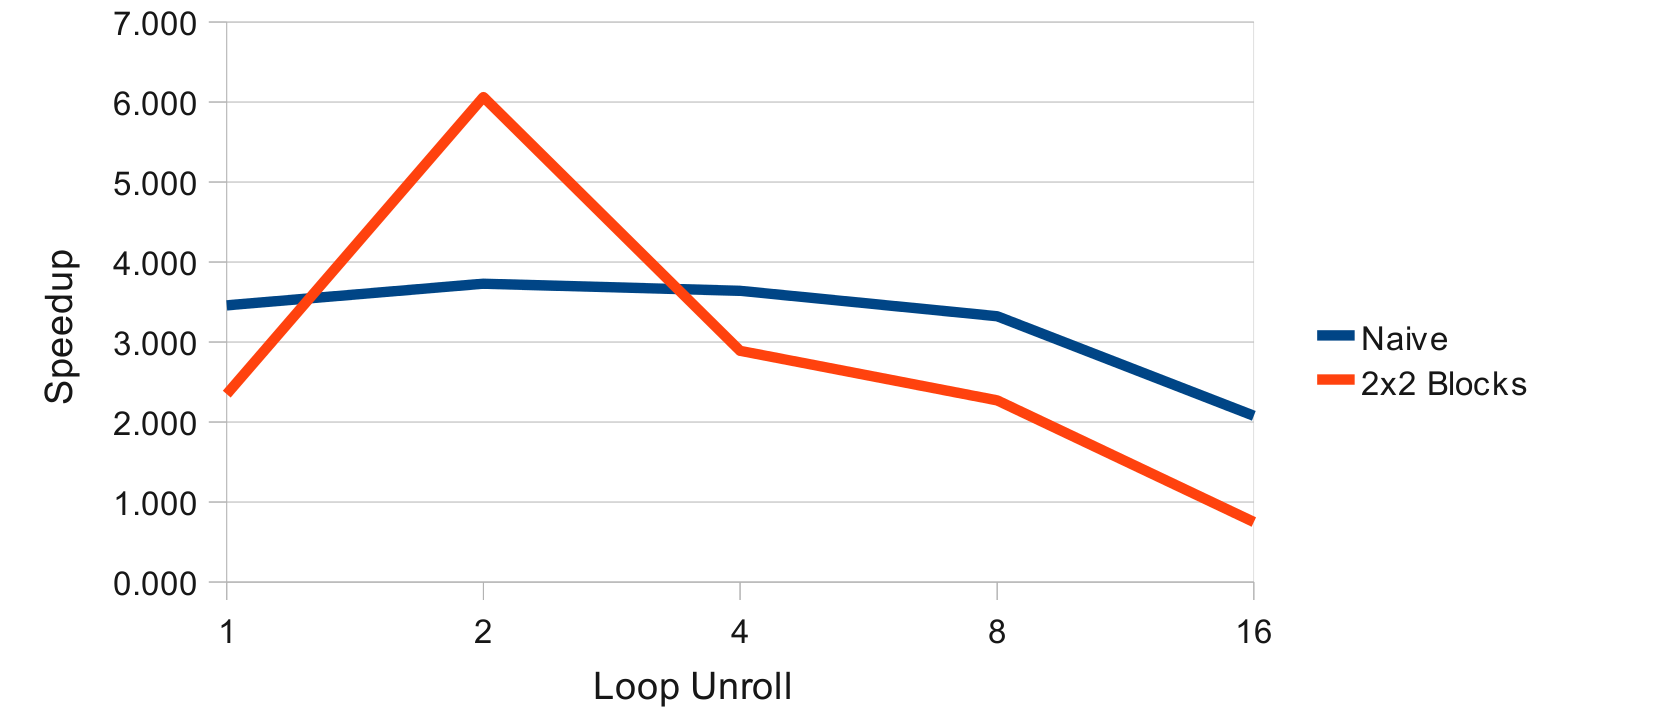
\includegraphics[clip]{unrolling}
\end{center}
\caption{Performance of 4k Matrix Multiplication with Unrolled Loops}\label{unroll}
\end{figure}

These measurements clearly show that value specialization provides
significant speedups over a non-specialized OpenCL kernel. This result
can be explained by the fact taht providing constant values at compile
time allows the OpenCL C compiler to do extensive constant
propagation-based optimizations.

The results from loop unrolling are more complicated. Unrolling loops
too much drastically decrease performance, most likely due to the
exhaustion of registers on the GPU device. Still, when properly tuned,
loop unrolling provides significant speedups allowing the blocked
Bacon kernel to beat the hand vectorized OpenCL kernel by nearly 30
percent.

\section{Stereo Disparity in Bacon}

In order to demonstrate that Bacon is suitable for complex
applications we consider an implementation of stereo disparity
matching. This is an application that is well suited to GPU
implementation due to being computationally expensive and naturally
parallel. The stereo disparity computation is significantly more
complex than matrix multiplication, requiring multiple steps such that
the entire process can not easily be implemented as a single kernel.

The stereo disparity matching problem is to generate a disparity image
given a pair of images from a stereo camera rig. Each pixel ($y,x$) in
the disparity image has a value ($v$) specifying a pixel offset that
matches the pixel at ($y,x$) in the left image to the pixel at
($y,x+v$) in the right image. These matched pixels correspond to the
same physical point in scene viewed by the cameras. This disparity
image can then be used to compute depth information and create a 3D
point cloud describing the scene, which is useful in a variety of
practical applications like robotics.

The stereo disparity method implemented used the Census
transform\cite{zabih:1994} both with simple local window matching and
with a partial implementation of the semi-global matching (SGM) technique
described by Hirschmuller\cite{hirschmuller:2005}. Testing during
development was done on sample image pairs from the Middlebury 2005
Stereo Dataset\cite{hirschmuller:2005}. Both a CPU implementation and
a Bacon implementation were written.

Although a complete implementation of the SGM algorithm was not
completed and neither Bacon implementation has been properly
optimized, the results are promising. The simple local window matcher
in Bacon produces the same output as the CPU version. The partial SGM
implementation produces a more accurate disparity image but takes
longer to run.

Including specialization time, the Bacon version of the local window
matcher takes almost as much time as the CPU version, but on
subsequent calls it takes less than 0.2 seconds which is more than a
10x speedup. This provides a good example of the practicality of the
value specialization mechanism; for processing video an extra
computation cost on the first frame will be quickly amortized over
subsequent frames.

\section{Future Work}

The Bacon system could benefit from a number of extensions to improve
its performance, generality, and utility to developers. One obvious
area of improvement would be to automatically determine the best
factor for loop unrolling rather than expecting it to be tuned
manually. The unrolling analysis could also be extended to the
implicit parallel ``loops'' created by the range of the computation;
optimally, it should be possible to generate kernels like the blocked
matrix multiplication shown from the naive matrix multiplication
kernel. Another simple improvement would be to perform strip mining
(Wolfe \cite{wolfe:1996}, section 9.8) and generate explicit vector
code for loops.

Just in time specialization as a method to improve performance on
parallel computations seems very promising in general, but there are
some limitations imposed by the use of OpenCL as a compiler target. An
implementation of this technique targeting a parallel processor at a
lower level would allow for more flexibility and much faster
specialization times.

\section{Conclusion}

We have shown that Bacon allows a high performance GPU matrix
multiplication kernel to be written in a naive style and executed with
nearly the performance of a hand-vectorized OpenCL kernel due to the
performance benefits of just in time specialization. Further, we have
shown that by re-writing that kernel with a generalized block strategy
and selecting appropriate loop unrolling settings, the performance of
the hand vectorized OpenCL kernel can be exceeded.

We are distributing this tool in the hope that it will be practically
useful for developing kernels targeting OpenCL compatible GPU devices.

\bibliography{bacon}{} 
\bibliographystyle{splncs03}
\end{document}
